%======================================================================
%   Zak Webb
%   Ph. D. Thesis
%   Department of Physics and Astronomy
%   University of Waterloo
% 
%   Universality of single-particle scattering
%======================================================================


\documentclass[../thesis-main/thesis-main]{subfiles}
\begin{document}

\chapter{Universality of Quantum Walk}
\label{chap:SP_universality}

%%%%%%%%%%%%%%%%%%%%%%%%%%%%%%%%%%%%%%%%%%%%%%%%%%%%%%%%%%%%%%%%%

Quantum walk is an intuitive framework for developing quantum algorithms, inspired by the classical model of random walk.  This framework has lead to examples of exponential speedups over classical computation \cite{CCDFGS03}, as well as optimal algorithms for element distinctness \cite{Amb07} and formula evaluation \cite{FGG08}.  Additionally, the framework of \chap{scattering_on_graphs} can be thought of as a special kind of continuos-time quantum walk.

With all of these algorithmic uses, we would then wonder at the computational power of this model.  Using the ideas of graph scattering, Childs \cite{Chi09} was able to show that the model of continuous time quantum walk is universal for quantum computation (and later showed the same for discrete-time quantum walk \cite{Chi10}).  This chapter will also show this result, but with a slightly different proof technique.

In particular, we will use results on the scattering behavior of finite-length wave-packets to implement single gates, and we will then show how to compose these scattering events for an entire computation.  This chapter is really a primer for \chap{MP_universality}, as many of the proof-techniques and ideas of this chapter will be used for the multi-particle case as well.

Most of this chapter will be devoted to showing how to simulate a circuit of a given form via graph scattering.

\todo{Move wavepacket propagation to this chapter?}


%%%%%%%%%%%%%%%%%%%%%%%%%%%%%%%%%%%%%%%%%%%%%%%%%%%%%%%%%%%%%%%%%


\section{Single qubit simulation}\label{sec:single_qubit_computations}

With our eventual goal of simulating an entire circuit via graph scattering, we will first need to understand how to perform single-qubit computations.  We will use many of the results of \chap{scattering_on_graphs}, and show that specific scattering behavior can be used as a computational tool.  This section will first encode the qubit, then show how to have a simulate a single gate, and finally show how to simulate multiple single-qubit gates.   These results will then be generalized for multiple-qubits in \sec{multi_qubit_computations}, and will be used nearly verbatim in \chap{MP_universality}.

%%%%%%%%%%%%%%%%%%%%%%%%%%%%

\subsection{Single qubit encoding}\label{sec:single_qubit_encoding}

In our search for simulations, we will first need to encode the logical state into some graph state.  We can then take inspiration from the current literature, or else see motivation from classical asynchronous systems, to encode our logical system via dual-rails.  In particular, a single qubit will correspond to two infinite paths, with a single wave-packet at specified momentum $k$ traveling along one of the two paths.  If the particle is located on the first (top) path, then the encoded qubit is in the logical state $\ket{0}$, while if the particle is on the second (bottom) path then the encoded qubit is in the logical state $\ket{1}$.  Schematically, this can be seen in \fig{wavetrain_encoding}.

\todo{change figure to Gaussian as opposed to square?}

\begin{figure}
  \centering
  \subfloat[][]{ 
    \tikzsetnextfilename{SP_u_wavetrain0}
    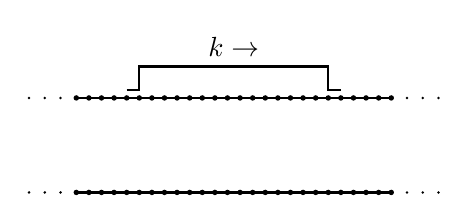
\begin{tikzpicture}[
  vert/.style={circle,fill=black,inner sep=.7pt,minimum width=0pt},
  dots/.style={circle,fill=black,inner sep=.25pt,minimum width=0pt},
  thick,
  scale=0.4]
  \foreach \x in {0,.4,...,10}{
    \node at (\x ,0) [vert]{};
    \node at (\x ,3) [vert]{};
  }

  \draw (0,0) -- (10,0);
  \draw (0,3) -- (10,3);

  \begin{scope}[yshift=0cm]
  \draw (1.6,3.25) -- (2,3.25) -- (2,4) to node [above] {$k\rightarrow$}
        (8,4) -- (8,3.25) -- (8.4,3.25);
  \end{scope}

  \foreach \xsh in {-1.5cm , 10.5cm}{
  \foreach \ysh in {0cm, 3cm}{
    \begin{scope}[xshift=\xsh,yshift=\ysh]
      \node at (0,0) [dots]{};
      \node at (0.5,0) [dots] {};
      \node at (1,0) [dots]{};
    \end{scope}
  }}
\end{tikzpicture}
    \label{fig:wavetrain0}
  }
  \qquad
  \subfloat[][]{
    \tikzsetnextfilename{SP_u_wavetrain1}
    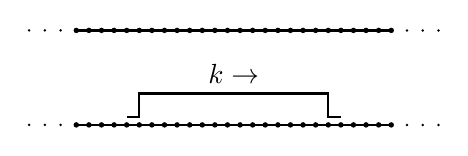
\begin{tikzpicture}[
  vert/.style={circle,fill=black,inner sep=.7pt,minimum width=0pt},
  dots/.style={circle,fill=black,inner sep=.25pt,minimum width=0pt},
  thick,
  scale=0.4]
  \foreach \x in {0,.4,...,10}{
    \node at (\x ,0) [vert]{};
    \node at (\x ,3) [vert]{};
  }

  \draw (0,0) -- (10,0);
  \draw (0,3) -- (10,3);

  \begin{scope}[yshift=-3cm]
  \draw (1.6,3.25) -- (2,3.25) -- (2,4) to node [above] {$k\rightarrow$}
        (8,4) -- (8,3.25) -- (8.4,3.25);
  \end{scope}

  \foreach \xsh in {-1.5cm , 10.5cm}{
  \foreach \ysh in {0cm, 3cm}{
    \begin{scope}[xshift=\xsh,yshift=\ysh]
      \node at (0,0) [dots]{};
      \node at (0.5,0) [dots] {};
      \node at (1,0) [dots]{};
    \end{scope}
  }}
\end{tikzpicture}
    \label{fig:wavetrain1}
   }
  \caption{A qubit is encoded using single-particle wave packets at momentum $k$.  \subfig{wavetrain0} An encoded $\ket{0}$.  \subfig{wavetrain1} An encoded $\ket{1}$.}
  \label{fig:wavetrain_encoding}
\end{figure}

If we didn't mind using an infinite Hilbert space to encode our qubits, we could actually use the eigenstates of the two paths to correspond to the two logical states, but we will eventually want to assume that the encodings have a well-defined position in space to ensure that we need only measure a (relatively) small number of qubits in order to determine the location of the particle with high probability.  To ensure this localization in space (and to use some of our error bounds on the time evolution), we will assume that the logical states are encoded using a truncated Gaussian wave-packet, with four attributes that specify the state: the momentum $k$, the standard deviation $\sigma$, the center of mass $\mu$, and the cutoff range $L$ (which will be closely related to $\sigma$).  With these four values, and assuming that the vertices of the infinite path are labeled as $(x,z)$ for $x\in \ZZ$ and $z\in \FF_2$, we then have that the logical qubit in our system will be encoded into the states
\begin{align}
  \ket{z}_{\text{log}} = \gamma \sum_{x = \mu - L}^{\mu + L} e^{ i k x} e^{ - \frac{(x-\mu)^2}{2\sigma^2}} \ket{x,z} \label{eq:single_qubit_encoding}.
\end{align}
It is important to realize that none of these four values depend on the value of the encoded qubit; this will allow us to interfere the wave-packets arising from different paths to the same computational basis path as there will be no extraneous information about the logical state.

This encoding is specifically chosen so that we can use \thm{single_particle_wavepacket_bound}, and guarantee various attributes about the time evolution of such systems.

%%%%%%%%%%%%%%%%%%%%%%%%%%%%

\subsection{One single-qubit unitary}

With an actual encoding of a logical qubit, the next step will be to apply an encoded unitary to the logical state.  However, our current encoding is on two (disconnected) paths, and as such if we want to apply any unitary that mixes amplitudes among the two basis states we somehow need to connect the two paths. (Unitaries diagonal in the computational basis will use the same formalism, but they have additional constraints that might make them easier to apply.)


Note that \chap{scattering_on_graphs} was all about connecting (semi-) infinite paths, where the amplitudes move from one path to another.  As hinted in the chapter, we can implement encoded unitaries in this manner, if we restrict ourselves to specific momenta and specific scattering gadgets.  Namely, we will examine graphs $\widehat{G}$ with four terminal vertices such that at the momentum $k$ encoding the qubits, the scattering matrices take the form
\begin{align}
  S(k) &= \begin{pmatrix} 0 & U^{T} \\
  U & 0\end{pmatrix},
  \label{eq:unitary_s_matrix}
\end{align}
where $U$ is a specific $2\times 2$ unitary matrix.  This will then allow us to apply the unitary $U$ to the encoded qubit.

More explicitly, we will have four semi-infinite paths, and we will label the four paths by $0_{\text{in}}$, $1_{\text{in}}$, $0_{\text{out}}$, and $1_{\text{out}}$ (where this labeling is the same as in equation \eq{unitary_s_matrix}).  We assume that the wave-packet encoding a qubit travels toward the graph $\widehat{G}$ along the two paths $0_{\text{in}}$ and $1_{\text{in}}$.  Far from the graph the evolution of this wavepacket is nearly identical to that of an infinite path, and thus our encoded qubit is well defined.  As the wavepacket scatters through the graph $\widehat{G}$, the state of the qubit is not well defined, but after scattering, most of the amplitude is on the $0_{\text{out}}$ and $1_{\text{out}}$ paths, and is in the form of an encoded qubit. 

For specific $\mu$, $L$, $\sigma$, and $t$, we the have from \thm{single_particle_wavepacket_bound} that the outgoing wave-packet for the two computational basis states is well approximated by the wave-packet corresponding to the state $U \ket{z}$.  If we remember that the form of the wave-packet doesn't depend on the value of the initial encoded qubit, we can see that the evolution of the two basis states interfere, and thus for \text{any} encoded state $\ket{\phi}$, the outgoing wavepacket is well approximated by the encoded $U\ket{\phi}$.  This is exactly what we were looking for.


\todo{make graph?}


%%%%%%%%%%%%%%%%%%%%%%%%%%%%

\subsection{Evolution on a finite graph}


Unfortunately, a single unitary will not be sufficient for our purposes; while we could probably find a four-terminal graph that computes whether a given circuit accepts or rejects its input, most of the computation would be found in the construction of the underlying graph, as opposed to the evolution itself.  To ensure that the computational power arises from the time evolution of the system, we will need to place multiple graphs as scattering obstacles for the computation.  This causes problems, though, in that we extensively utilize the semi-infinite paths in our analysis; we somehow need to truncate the graph while maintaining our results about the time-evolution.

To do this, we will apply our truncation lemma (\lem{truncation}), as it was designed specifically for this reason.  Assuming that two Hamiltonians are identical on some set of basis states, and assuming that the support of the initial state is far (in some specified sense) from the difference, then the evolution of the state is the same for the two Hamiltonians, up to a small error term.  By using this lemma on the scattering graph with semi-infinite paths, we can then see that if the paths are long enough (as compared to the location of the initial state), then the evolution of an initial wave-packet is relatively unchanged by the removal of the far vertices.  Basically, \lem{truncation} will allow us to prove an analog of \thm{single_particle_wavepacket_bound} for finite graphs.

\begin{figure}
  \centering
  \tikzsetnextfilename{SP_u_single_qubit_scattering_graph}
  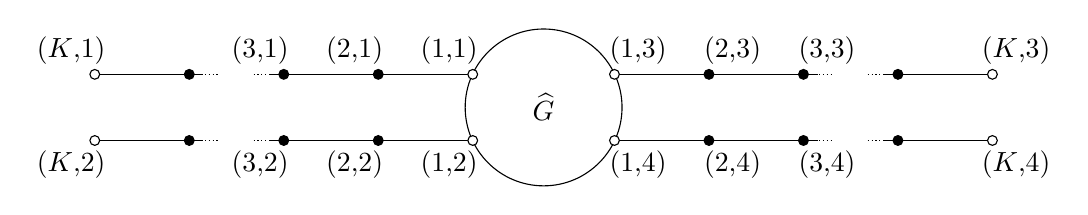
\begin{tikzpicture}[scale = 1.2,
    thin,
    attach/.style={circle,fill=white,draw=black,
      inner sep=1.25pt,minimum size=0pt},
    vert/.style={circle,draw=black,fill=black,
      inner sep=1.25pt,minimum size=0pt},
    attach/.style={circle,draw=black,fill=white,
      inner sep=1.25pt,minimum size=0pt},
    dots/.style={circle,fill=black,
      inner sep=.5pt,minimum size=0pt}]
      

   \draw (4.75,.35) circle (.83) node {$\widehat{G}$};

   \foreach \y in {0,.7}{
   \begin{scope}[yshift = \y cm]
   \draw (0,0) -- (1.15,0);
   \draw[densely dotted] (1,0) -- (1.32,0);
   \draw[densely dotted] (1.68,0) -- (2,0);
   \draw (1.85,0) -- (4,0);
   \begin{scope}[xshift=-.5cm]
   \draw (6,0) -- (8.15,0);
   \draw[densely dotted] (8,0) -- (8.32,0);
   \draw[densely dotted] (8.68,0) -- (9,0);
   \draw (8.85,0) -- (10,0);
   \end{scope}
   \foreach \x in {1,2,3,6.5,7.5,8.5}{
   \node at (\x, 0) [vert] {};}

   \node at (4,0) [attach] {};
   \node at (5.5,0) [attach]{};
   \node at (0,0) [attach] {};
   \node at (9.5,0) [attach] {};
   

   \end{scope}}
   
   
   \node[anchor=north] at (3.75,0) {(1,2)};
   \node[anchor=north] at (2.75,0) {(2,2)};
   \node[anchor=north] at (1.75,0) {(3,2)};

   \node[anchor=north] at (-.25,0) {($K$,2)};
   
   \node[anchor=south] at (3.75,.7) {(1,1)};
   \node[anchor=south] at (2.75,.7) {(2,1)};
   \node[anchor=south] at (1.75,.7) {(3,1)};

   \node[anchor=south] at (-.25,.7) {($K$,1)};
   
   \node[anchor=south] at (5.75,.7) {(1,3)};
   \node[anchor=south] at (6.75,.7) {(2,3)};
   \node[anchor=south] at (7.75,.7) {(3,3)};

   \node[anchor=south] at (9.75,.7) {($K$,3)};
      
   \node[anchor=north] at (5.75,0) {(1,4)};
   \node[anchor=north] at (6.75,0) {(2,4)};
   \node[anchor=north] at (7.75,0) {(3,4)};

   \node[anchor=north] at (9.75,0) {($K$,4)};
\end{tikzpicture}
  \caption{A graph $G(K)$ used to perform a single-qubit gate on an encoded qubit. 
  \label{fig:single_qubit_scattering_graph}}
\end{figure}

More concretely, let $H=A(G)$ be the Hamiltonian for a single particle scattering off of a finite graph $\widehat{G}$ with $N$ paths.  Let $G(K)$ be the finite graph obtained from $G$ by truncating each of the paths to have a total length $K$ (so that the endpoints of the paths are labeled $(K,j)$ for $j\in [N]$), and choose $\widetilde{H}=A(G(K))$ (see \fig{single_qubit_scattering_garph}). Let the subspace $\mathcal{K}$ be spanned by basis states corresponding to vertices in $G(K)$.  Choose a momentum $k\in (-\pi,0)$, a position $\mu$, and a cutoff length $L$, and let $|\Phi\rangle=|\psi^j(0)\rangle$ be the same initial state as in \thm{single_particle_scattering_bound}.  We will choose the evolution time $T$ so that for $0\leq t\leq T$, the time-evolved state remains far from the vertices labeled $(K,j)$ (for each $j\in\{1,\ldots,N\}$), and thus far from the effect of truncating the paths.  Note that this requires $K > \mu + L$.  More precisely, we will choose $T=\OO(L)$ and $K = \OO(L)$ so that, for times $0\leq t\leq T$, the state $|\alpha^j (t)\rangle$ from \thm{single_particle_wavepacket_bound} has no amplitude on vertices within a distance $N_0=\Omega(L)$ from the endpoints of the paths. For such times $t$ we have
\begin{align}
\left(1-P\right)H^r |\alpha^j \left(t\right)\rangle=0 \text{ for all } 0\leq  r < N_0,
\end{align}
where $P$ is the projector onto $\mathcal{K}$.   With these values, we can apply \lem{truncation} where $W=H=A(G)$, $|\gamma(t)\rangle=|\alpha^j(t)\rangle$, and the bound $\delta=\OO(\sqrt{\log L/L})$ from \thm{single_particle_wavepacket_bound}. The lemma then says that, for times $t$ such that $0\leq t\leq T$,
\begin{equation}
  \big\Vert \left(e^{-iA(G) t}-e^{-iA(G(K))t}\right)|\psi^{j}(0)\rangle \big\Vert=\OO\Bigg(\sqrt{\frac{\log L}{L}}\Bigg)
\end{equation}
so, for $0\leq t\leq T$, when combined with \thm{single_particle_wavepacket_bound}, we can see
\begin{align}
  \big\Vert e^{-iA(G(K)) t}|\psi^{j}(0)\rangle-|\alpha^{j}(t)\rangle \big\Vert =\OO\Bigg(\sqrt{\frac{\log L}{L}}\Bigg).
    \label{eq:trunc_paths}
\end{align}
In other words, for small enough evolution times, the conclusion of \thm{single_particle_wavepacket_bound} still holds if we replace the full Hamiltonian $A(G)$ with the truncated Hamiltonian $A(G(K))$ (albeit with a larger constant).  Note that this analysis is rather informal, and is more to give an intuition for the more exact analysis.

With the guaranteed bounds on the scattering behavior for finite graphs, we can give explicit bounds on the time-evolution of encoded qubits.  In particular, let us assume that $\widehat{G}$ is a four-terminal gadget used to implement a unitary $U$ at momentum $k$, and let us assume that our initial states are encoded as Gaussian wave-packets a distance $\mu$ from the graph, with a cutoff distance $L$.  We will give explicit values of $K$, along with $\mu$ and $L$, so that the scattering event will cause the unitary $U$ to be applied to the encoded qubits, along with bounds on the error term.



\todo{is this the correct $\sigma$ definition?}

Explicitly, assuming that the four paths are labeled as in \fig{single_qubit_scattering_graph}, where $0_\text{in}$, $1_{\text{in}}$, $0_{\text{out}}$ and $1_{\text{out}}$ are labeled as $1$, $2$, $3$, and $4$, respectively, we have that our input logical basis states are
\begin{align}
  \ket{z}_{\text{log},\text{in}} = \gamma \sum_{x = \mu - L}^{\mu + L} e^{ i k x} e^{ - \frac{(x-\mu)^2}{2\sigma^2}} \ket{x,z+1},
  \label{eq:single_qubit_input_encoding}
\end{align}
where we assume that $\sigma = \frac{L}{2\sqrt{\log L}}$, as in \thm{single_particle_wavepacket_bound}.  Further, we can make us of the theorem, noting that $\ket{z}_{\text{log},\text{in}}$ are of the form $\ket{\alpha^{z+1}(0)}$, to define output logical states as well:
 \begin{align}
  \ket{z}_{\text{log},\text{out}} = \gamma e^{- 2 i T \cos k} \sum_{x = \mu - L}^{\mu + L} e^{ -i k x} e^{ - \frac{(x-\mu)^2}{2\sigma^2}} \ket{x,z+3},
  \label{eq:single_qubit_output_encoding}
\end{align}
where $T = \frac{\mu}{\sin |k|}$.  Note that the momentum $k$ for the output logical states implies that the particles are moving away from the graph $\widehat{G}$.  In addition to these logical basis states, we can define logical superpositions for a state $\ket{\psi} = \alpha \ket{0} + \beta\ket{1}$ as
\begin{align}
  \ket{\psi}_{\text{log},\text{in}} = \alpha \ket{0}_{\text{log},\text{in}} + \beta \ket{1}_{\text{log},\text{in}}
\end{align} 
and
\begin{align}
  \ket{U \psi}_{\text{log},\text{out}} = \big(\alpha U_{00} + \beta U_{01} \big) \ket{0}_{\text{log},\text{out}} + \big(\alpha U_{10} + \beta U_{11} \big)\ket{1}_{\text{log},\text{out}}.
\end{align}
With these definitions, we will want to show that the input states evolve to the corresponding output states, in a manner similar to \thm{single_particle_wavepacket_bound}.  Working through the math, we then find:

\todo{Run through proof, ensure correct}

%%%%%%%%%%%%%%%%%%%%%%%%%%%%%%%%
% Lemma for single-qubit single unitary computation
\begin{lemma}
\label{lem:single_qubit_encoded_computation}
  Let $k\in (-\pi,0)$, and let $\widehat{G}$ be a four-terminal gate gadget, such that its scattering matrix at momentum $k$ is of the form \eq{unitary_s_matrix}.  Letting the logical states $\ket{z}_{\text{log},\text{in}}$ and $\ket{z}_{\text{log},\text{out}}$ be defined as in \eq{single_qubit_input_encoding} and \eq{single_qubit_output_encoding}, where $\mu \geq 2L $ and $K \geq \frac{5 \mu}{3}$ and $T = \frac{\mu}{\sin |k|}$, we have that there exists some constant $\xi$ such that for all $0 \leq t \leq T$
\begin{align}
  \Big\Vert e^{i A(G(K))t} \ket{\phi(0)} - \ket{\phi(t)} \Big\Vert \leq \xi \sqrt{\frac{\log L}{L}},
\end{align}
where
\begin{align}
  \ket{\phi(t)} = \alpha \ket{\alpha^{1}(t)} + \beta \ket{\alpha^2(t)},
\end{align}
and the $\ket{\alpha^j(t)}$ are as defined in \thm{single_particle_wavepacket_bound}.  In particular, we have
\begin{align}
  \Big\Vert e^{i A(G(K)) T} \ket{\psi}_{\text{log},\text{in}} - \ket{U\psi}_{\text{log},\text{out}} \Big\Vert \leq \xi \sqrt{\frac{\log L}{L}}.
\end{align}
\end{lemma}

\begin{proof}
Note that
\begin{align}
  &\Big\Vert e^{i A(G(K))t} \ket{\phi(0)} - \ket{\phi(t)} \Big\Vert \nonumber\\
  &\qquad\leq |\alpha| \Big\Vert e^{i A(G(K))t} \ket{\alpha^1(0)} - \ket{\alpha^1(t)}\Big\Vert
  + |\beta| \Big\Vert e^{i A(G(K))t}  \ket{\alpha^2(0)} - \ket{\alpha^2(t)}\Big\Vert .
\end{align}
We now have nearly have the form of the bound in \thm{single_particle_wavepacket_bound}, but where we use truncated paths.  

We will use \lem{truncation}, with $H = A(G)$, $\tilde{H} = A(G(K))$, and $N_0 = K - \mu - L \geq \frac{\mu}{6}$, and where the error bound $\delta = \chi \sqrt{\frac{\log L}{L}}$ comes from \thm{single_particle_wavepacket_bound}.  Assuming that $L$ is taken large enough so that $\delta < 1$, the lemma then gives us that for all $0 \leq t \leq T$,
\begin{align}
  \Big \Vert \big(e^{- i A(G) t} - e^{- i A(G(K))t}\big)\ket{\alpha^j(0)}\Big\Vert \leq \bigg( \frac{4 e \Vert A(G) \Vert t}{\mu - 2 - L} + 2 \bigg) \bigg[ \chi \sqrt{\frac{\log L}{L}} + 2^{- \mu + L +2} \bigg(1 -   \chi \sqrt{\frac{\log L}{L}}  \bigg)\bigg].
\end{align}
If we then note that $\Vert A(G)\Vert$ is bounded by the maximum degree of the graph $G$ (a constant), and that $\mu - L - 2 \geq 3 \mu$, we then have 
 \begin{align}
  \Big \Vert \big(e^{- i A(G) t} - e^{- i A(G(K))t}\big)\ket{\alpha^j(0)}\Big\Vert \leq \bigg( \frac{12 e d }{\mu }\frac{\mu}{\sin |k|} + 2 \bigg)  (\chi +1)\sqrt{\frac{\log L}{L}}  \leq \zeta \sqrt{\frac{\log L}{L}}, 
\end{align}
where $\zeta$ is a constant (but does depend on $k$ and the graph $\widehat{G}$).

We can then combine these results, as
\begin{align}
  &\Big\Vert e^{i A(G(K))t}  \ket{\alpha^j(0)} - \ket{\alpha^j(t)}\Big\Vert \nonumber \\
  &\qquad\leq \Big\Vert\big( e^{i A(G(K))t}  - e^{ i A(G) t}\big)\ket{\alpha^j(0)} \Big\Vert  + \Big\Vert e^{i A(G)t}  \ket{\alpha^j(0)} - \ket{\alpha^j(t)}\Big\Vert   \leq \big(\chi + \zeta \big) \sqrt{\frac{\log L}{L}}.
\end{align}
From this, we can then see that
\begin{align}
  &\Big\Vert e^{i A(G(K))t} \ket{\phi(0)} - \ket{\phi(t)} \Big\Vert \nonumber\\
  &\qquad\leq |\alpha| \Big\Vert e^{i A(G(K))t} \ket{\alpha^1(0)} - \ket{\alpha^1(t)}\Big\Vert
  + |\beta| \Big\Vert e^{i A(G(K))t}  \ket{\alpha^2(0)} - \ket{\alpha^2(t)}\Big\Vert \\
  & \qquad \leq \big( |\alpha| + |\beta| \big) \big( \chi + \zeta \big)  \sqrt{\frac{\log L}{L}},
\end{align}
and by setting $\xi = \sqrt{2}(\chi + \zeta)$ we have the requisite bound (for large enough $L$).

If we then note that $\phi(0) = \ket{\psi}_{\text{log},\text{in}}$ and $\phi(T) = \ket{U \psi}_{\text{log},\text{out}}$, we also have the particular bound we were looking for.
\end{proof}

Essentially, \lem{single_qubit_encoded_computation} tells us that even when truncated to finite length paths, the scattering events on our graphs apply an encoded unitary to the logical states.  This is represented pictorially in \fig{single_particle_cartoon}.
 

\todo{correct \fig{single_particle_cartoon}.}

\begin{figure}
  \centering
  \tikzsetnextfilename{SP_u_single_particle_cartoon}
  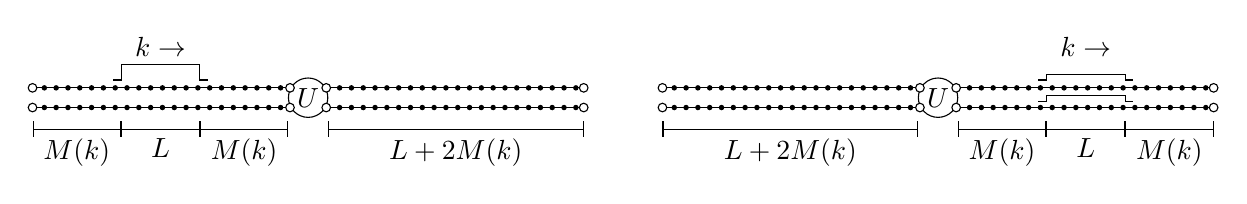
\begin{tikzpicture}[
  scale = 0.5,
  unitary/.style={circle,draw=black,fill=white,
    inner sep=0pt,minimum size=5mm},
  verts/.style={circle,fill=black,inner sep=.7pt,minimum size=0},
  attach/.style={circle,fill=white,draw=black,inner sep=1.1pt,minimum size=0pt}]
  \draw (-2,0.25) to (12,0.25);
  \draw (-2,-0.25) to (12,-0.25);

  \foreach \x in {-2,-1.7,...,12}{
  \foreach \y in {-.25,.25}{
    \node at (\x,\y) [verts] {};
  }}

  \node (1) at (5,0) [unitary] {$U$};

  \draw[xshift=-1cm] (1.05,.45) to (1.25,.45) to (1.25,.85) to (3.25,.85) 
           to (3.25,.45) to (3.45,.45);

  \node (momentum) at (1.25,1.3) [] {$k\rightarrow$};

  \draw[|-|] (-2,-.8)   to node[below] {$M(k)$} (0.25,-.8);
  \draw[|-|] (0.25,-.8) to node[below] {$L$}   (2.25,-.8);
  \draw[|-|] (2.25,-.8) to node[below] {$M(k)$} (4.5,-.8); 

  \draw[|-|] (5.5,-.8) to node[below] {$L + 2M(k)$} (12,-.8);

  \foreach \x in {-2, 12, 4.54, 5.46}{
  \foreach \y in {-.25, .25}{  
    \node at (\x,\y) [attach]{};
  }}

\begin{scope}[xshift=4cm]
  \draw (10,0.25) to (24,0.25);
  \draw (10,-0.25) to (24,-0.25);
  
  \foreach \x in {10,10.3,...,24}{
  \foreach \y in {-.25,.25}{
    \node at (\x,\y) [verts] {};
  }}
  
  \node (2) at (17,0) [unitary] {$U$};
 
  \draw[xshift=1cm] (18.55,.45) to (18.75,.45) to (18.75,.6)
     to (20.75,.6) to (20.75,.45) to (20.95,.45);

  \draw[xshift=1cm] (18.55,-.1) to (18.75,-.1) to (18.75,.05)
     to (20.75,.05) to (20.75,-.1) to (20.95,-.1);

  \node (momentum2) at (20.75,1.3) [] {$k\rightarrow$};


  \draw[|-|] (10,-.8) to node[below] {$L+2M(k)$} (16.5,-.8);
  \draw[|-|] (17.5,-.8) to node[below] {$M(k)$} (19.75,-.8);
  \draw[|-|] (19.75,-.8) to node[below] {$L$} (21.75,-.8);
  \draw[|-|] (21.75,-.8) to node[below] {$M(k)$} (24,-.8);
  
  \foreach \x in {10, 24, 16.54, 17.46}{
  \foreach \y in {-.25, .25}{  
    \node at (\x,\y) [attach]{};
  }}
\end{scope}
\end{tikzpicture}
  \caption{A single-qubit gate $U$ acts on an encoded qubit. The wave packet starts on the paths on the left-hand side of the figure, a distance $M(k)$ from the ends of the paths. After time $t_{\mathrm{I}}={3L}/{2}$ the logical gate has been applied and the wave packet has traveled a distance $2M(k)+L$ (up to error terms that are bounded as $\O(L^{-{1}/{4}}))$.}
  \label{fig:single_particle_cartoon}
\end{figure}

%%%%%%%%%%%%%%%%%%%%%%%%%%%%

\subsection{Multi-gate computations}\label{sec:single_qubit_multi_gate_computation}

\todo{start from here}

Now that we have a good approximation for the time evolution of a scattering event on a finite-sized graph, we can now expand our results to multiple scattering events.  To apply multiple unitaries, we will simply repeat the graph for a single unitary


With our analysis of an encoded single-qubit's evolution for one scattering event on a finite graph, we should be able to analyze multiple scattering events, corresponding to a circuit of some finite length.  In particular, if we want to apply multiple unitaries to a single qubit, we can place the corresponding scattering gadgets $\widehat{G}_i$ in series, and then connect the outputs of $\widehat{G}_i$ to the inputs of $\widehat{G}_{i+1}$ by a path of length $K - 2$.  We can then use \lem{truncation} to analyze each scattering event in series, using the output logical state of the $i$th scattering event for the input logical state of the $(i+1)$th scattering event.

\todo{make a figure}

Let us assume that a single-qubit circuit $\mathcal{C}$ is composed of $g$ unitaries, where the $i$th unitary applied is given by $U_i$.  Moreover, let us assume that at a momentum $k$, the graphs $\widehat{G}_i$ have scattering matrices of the form \eq{unitary_s_matrix} corresponding to the unitary $U_i$ (i.e., at momentum $k$, the graph $\widehat{G}_i$ implements an encoded $U_i$).  We can then construct a graph $G_{\mathcal{C}}$ which we will use to compute the circuit $\mathcal{C}$ using wave-packets at momentum $k$. 

\todo{technically, there is an off by one error with my bounds. Using the }

The graph $G_{\mathcal{C}}$ is constructed by combining the $G_i(K)$ into a single graph, where $G_i(K)$ is defined in \sec{single_qubit_single_gate_computation}.  We combine the $G_i(K)$ into a single graph by associating the output paths of $G_i(K)$ with the input paths of $G_{i+1}(K)$.  Assuming that the vertices of $G_i(K)$ are labeled as $(u,i)$, this essentially means that most of the vertices along the long paths have two labels, $(x,3, i)$ and $(K-x+1,1,i+1)$ or $(x,4,i)$ and $(K-x+1,2,i+1)$.  Equivalently, the graph $G_{\mathcal{C}}$ can be constructed by removing the input paths (paths $1$ and $2$) for all the $G_i(K)$ (except for $G_1(K)$), shorten each of the terminal paths by 1 (except for $G_g(K)$), and then connect the end of the paths for $G_i(K)$ to the input terminals of $G_{i+1}(K)$.

\todo{make a simple figure}

With this construction of $G_{\mathcal{C}}$, note that if we look only at the vertices supported within the copy of $G_i(K)$, we actually have the graph $G_i(K)$.  As such, we will be able to use \lem{truncation} and \lem{single_qubit_encoded_computation} to determine the evolution while a Gaussian wave-packet is located near the graph $\widehat{G}_i$.  If we assume that the initial wave-packet is located in the correct position near $\widehat{G}_i$, we can iteratively apply this idea, where the ``input'' logical state for the $(i+1)$th scattering event is simply the ``output'' from the $i$th scattering event.  As such, the logical state after the $g$th scattering event will correspond to the logical state after the circuit $\mathcal{C}$ has been applied.  

\todo{check this math}

Concretely, let us choose some cutoff length $L$, set $\sigma = \frac{L}{2\sqrt{\log L}}$, chose $\mu = 2L$ and $K = 2\mu$ and $T = \frac{\mu}{\sin |k|}$.  With these choices, our initial logical state will be nearly identical to \eq{single_qubit_input_encoding}, but where the basis states also have a label corresponding to fact that there are multiple long paths:
\begin{align}
  \ket{z}_{\text{log},\text{in}} = \gamma \sum_{x = \mu - L}^{\mu + L} e^{ i k x} e^{ - \frac{(x-\mu)^2}{2\sigma^2}} \ket{x,z+1,1}.
\end{align}
In a similar manner, the final state of the qubit will be defined as
 \begin{align}
  \ket{z}_{\text{log},\text{out}} = \gamma e^{- 2 i Tg \cos k} \sum_{x = \mu - L}^{\mu + L} e^{ -i k x} e^{ - \frac{(x-\mu)^2}{2\sigma^2}} \ket{x,z+3,g},
\end{align}
Additionally, we will need to define logical states at several times throughout the computation, corresponding to the states after each applied unitary.  As such, we will define the logical state after the $j$th scattering event (and before the $(j+1)$th scattering event) as
\begin{align}
  \ket{z}_{\text{log},j} &= \gamma e^{-2i Tj \cos k}\sum_{x = \mu - L}^{\mu + L} e^{ i k x} e^{ - \frac{(x-\mu)^2}{2\sigma^2}} \ket{x,z+1,j+1} \\
  &= \gamma e^{- 2 i Tj \cos k} \sum_{x = \mu - L}^{\mu + L} e^{ -i k x} e^{ - \frac{(x-\mu)^2}{2\sigma^2}} \ket{x,z+3,j}.
\end{align}

\todo{make the words work}
\begin{align}
  &\Big \Vert e^{ i A(G_{\mathcal{C}} )g T} \ket{\psi}_{\text{log},\text{in}} - \ket{U_{\mathcal{C}} \psi}_{\text{log},\text{out}}\Big \Vert\nonumber\\
  & \qquad \leq \sum_{j = 0}^{g-1} \Big \Vert e^{ i A(G_{\mathcal{C}})T} \ket{U_{j} U_{j-1}\cdots U_1 \psi}_{\text{log},j} - \ket{U_{j+1}U_{j} \cdots U_1 \psi}_{\text{log},j+1}\Big \Vert
\end{align}
Note that each individual term is close to that in \lem{single_qubit_encoded_computation}, but where the Hamiltonian is given by $A(G_{\mathcal{C}})$ as opposed to $A(G(K))$.  However, we can use \lem{truncation}, with $H = A(G_{\mathcal{C}})$, $\tilde{H} = G(K-1)$,  $N_0 = \frac{\mu}{4}$, and the error $\delta$ from \lem{single_qubit_encoded_computation}, we have that for all logical states $\ket{\phi}$,
\begin{align}
   &\Big \Vert e^{ i A(G_{\mathcal{C}})T} \ket{\phi}_{\text{log},j} - \ket{U_{j+1}\phi}_{\text{log},j+1}\Big \Vert\nonumber\\
   &\leq \Big(\frac{ 16 e \norm{A(G_{\mathcal{C}})} T}{\mu} + 2\Big)\bigg[ \xi \sqrt{\frac{\log L}{L}} + 2^{- \mu + L +2} \bigg(1 -   \chi \sqrt{\frac{\log L}{L}} \bigg)\bigg]\\
   & \leq \kappa_j \sqrt{\frac{\log L}{L}},
\end{align}
where $\kappa$ is depends on $k$ and the maximum degree of $G_{\mathcal{C}}$ (which we assume to be constant).  We can then see that
\begin{align}
  &\Big \Vert e^{ i A(G_{\mathcal{C}} )g T} \ket{\psi}_{\text{log},\text{in}} - \ket{U_{\mathcal{C}} \psi}_{\text{log},\text{out}}\Big \Vert\nonumber\\
  & \qquad \leq \sum_{j = 0}^{g-1} \Big \Vert e^{ i A(G_{\mathcal{C}})T} \ket{U_{j} U_{j-1}\cdots U_1 \psi}_{\text{log},j} - \ket{U_{j+1}U_{j} \cdots U_1 \psi}_{\text{log},j+1}\Big \Vert\\
  &\qquad \leq g\kappa \sqrt{\frac{\log L}{L}}.
\end{align}
As such, if we take $L$ larger than $g^2\kappa^2$ we find that the error can be made arbitrarily small, and thus we were able to simulate a single-qubit unitary via scattering.
\todo{figure out product log stuff}

%%%%%%%%%%%%%%%%%%%%%%%%%%%%

\subsection{Explicit encodings}\label{sec:explicit_encodings}

\todo{Find universal gate set for several momenta ($\pi/2$, $\pi/4$, $\pi/3$, etc.)}



%%%%%%%%%%%%%%%%%%%%%%%%%%%%%%%%%%%%%%%%%%%%%%%%%%%%%%%%%%%%%%%%%

\section{Multi-qubit computations}
\label{sec:multi_qubit_computations}

Now that we have a decent understanding of how to encode a single qubit computation via scattering, we now need to understand multi-qubit computations.  The intuitive construction will remain the same, but the requisite number of vertices will become rather large.  In particular, our construction will require an exponential number of long paths.  This exponential size is required, however, as the Hilbert space of a single-particle quantum walk is only as large as the number of vertices of the graph

Let us now give the encoding of $n$ qubits in our scattering framework.  As in \sec{single_qubit_encoding}, we will encode the state as a wave-packet traveling along an infinite path, where the value of the qubit is encoded in the path on which the particle is located.  For a single qubit, this meant that we had two infinite paths, corresponding to logical $0$ and $1$.  For $n$ qubits, however, this means that we need $2^n$ infinite paths, one path corresponding to each basis state.

We will still have four important quantities that are independent of the state of the qubit, namely the momentum of the wave-packet $k$, the position of the center of the wave-packet $\mu$ (which does depend on $t$), the cutoff distance $L$, and the standard deviation of the Guassian $\sigma$.  As such, if we label the $2^n$ infinite paths by the strings $\mathbf{z}\in \FF_2^n$, and the vertices as $(x,\mathbf{s})$ for $x\in \ZZ$ and $\mathbf{z}\in \FF_2^n$, we have that the logical states are encoded in the wave-packets
\begin{align}
  \ket{\mathbf{z}}_{\text{log}} = \gamma \sum_{x = \mu - L}^{\mu + L} e^{ i k x} e^{ - \frac{(x-\mu)^2}{2\sigma^2}} \ket{x,\mathbf{z}} \label{eq:multi_qubit_encoding}.
\end{align}
Note that we again use this construction so that we will be able to analyze the dynamics via \thm{single_particle_wavepacket_bound}.

%%%%%%%%%%%%%%%%%%%%%%%%%%%%

\subsection{Single gates}\label{sec:multi_qubit_single_gate}

Now that we have an encoding of our qubits, we will need to somehow apply encoded unitary gates.  We have already done most of the work in \sec{single_qubit_computations}, and we just need to show how to use the single-qubit results in our larger encoding, and how to perform multi-qubit entangling gates.

Our implementation of single-qubit unitaries for multi-qubit computations is to use many copies of the single-qubit implementation.  In particular, since a single qubit unitary $U$ acting on qubit $w\in [n]$ can be written as
\begin{align}
  \II_{2^{w-1}} \otimes U \otimes \II_{2^{n-w}} = \sum_{x \in \FF_2^{w-1}, y\in \FF_2^{n-w}} \ketbra{x}{x} \otimes U \otimes \ketbra{y}{y},
\end{align}
we can apply the unitary $U$ on the encoded $w$ qubit by ensuring that the scattering occurs for each computational basis state of the other qubits.  This means that by placing $2^{n-1}$ copies of the graph $\widehat{G}$ as obstacles in the paths, one for each computational basis state, the scattering behavior is exactly as expended.  

\todo{check whether errors add}

\todo{make multi qubit gate figure}


For multi-qubit entangling unitaries, the solution is even more simple; we simply relabel the output paths.  If we note that many multi-qubit gates such as a controlled-NOT gate or a Toffoli gate simply permutes the computational basis states, along with the fact that the particular path a particle travels along corresponds to its logical state, by relabeling the paths, or equivalently permuting the paths, we apply an encoded entangling gate.  Schematically, this can be seen in \fig{entangling_gate}.  Note that this method of applying a multi-qubit gate is independent of the encoding momenta, and thus can be used for all such momenta.  

Assuming that a given two-qubit unitary $V$ occurs after some single-qubit unitary $U$, we construct a graph implementing $VU$ by taking a copy of $G_U(K)$, and then permuting its output paths.  Note that this means that for a given copy of $\widehat{G}_j$, the logical states corresponding to the input paths might be different from the logical states corresponding to the output paths.

\todo{make \fig{entangling_gate} entangling gate}.


Explicitly, assuming that the $2^{n+1}$ paths are labeled as in \fig{multi_qubit_scattering_graph}, where the path for $z_{\text{in}}$ for $z\in \FF_2^n$ is labeled as $z+1$, while the $z_{\text{out}}$ are labeled as $z+2^n+1$, we have that our input logical basis states are
\begin{align}
  \ket{z}_{\text{log},\text{in}} = \gamma \sum_{x = \mu - L}^{\mu + L} e^{ i k x} e^{ - \frac{(x-\mu)^2}{2\sigma^2}} \ket{x,z+1},
  \label{eq:multi_qubit_input_encoding}
\end{align}
where we assume that $\sigma = \frac{L}{2\sqrt{\log L}}$, as in \thm{single_particle_wavepacket_bound}.  Note that this is identical to the sinlge particle case \eq{single_qubit_input_encoding}, but with more input paths.  We can then take inspiration from the single qubit case, and define the output logical states as well:
 \begin{align}
  \ket{z}_{\text{log},\text{out}} = \gamma e^{- 2 i T \cos k} \sum_{x = \mu - L}^{\mu + L} e^{ -i k x} e^{ - \frac{(x-\mu)^2}{2\sigma^2}} \ket{x,z+2^n + 1},
  \label{eq:multi_qubit_output_encoding}
\end{align}
where $T = \frac{\mu}{\sin |k|}$.  Note that the momentum $k$ for the output logical states implies that the particles are moving away from the graph $\widehat{G}$.  In addition to these logical basis states, we can define
\begin{align}
  \ket{\psi}_{\text{log},\text{in}} = \sum_{z\in \FF_2^n} \alpha_z \ket{z}_{\text{log},\text{in}}
\end{align} 
and
\begin{align}
  \ket{U \psi}_{\text{log},\text{out}} = \sum_{y,z\in\FF_2^N} U_{zy}\ket{z}_{\text{log},\text{out}},
\end{align}
where $U$ is thought of as a unitary on $n$ qubits.  With these definitions, we will want to show that the input states evolve to the corresponding output states.  This essentially follows from \lem{single_qubit_encoded_computation}, but where we need to do some small work showing that the errors don't grow like the number of paths.

\begin{corollary}
\label{cor:multi_qubit_single_gate_encoded_computation}
  Let $k\in (-\pi,0)$, let $\widehat{G}$ be a four-terminal gate gate, such that its scattering matrix at momentum $k$ is of the form \eq{unitary_s_matrix}, and let $V$ be a permutation of the underlying basis states.  Letting the logical states $\ket{z}_{\text{log},\text{in}}$ and $\ket{z}_{\text{log},\text{out}}$ be as in \eq{multi_qubit_intput_encoding} and \eq{multi_qubit_output_encoding}, where $\mu \geq 2L$ and $\frac{3\mu}{2} \leq K \leq 2\mu$ and $T = \frac{\mu}{\sin |k|}$, we have that there exists some constant such that for all $0 \leq t \leq T$, 
\begin{align}
  \Big\Vert e^{i A(G_V^n(K))t} \ket{\phi(0)} - \ket{\phi(t)} \Big\Vert \leq \xi \sqrt{\frac{\log L}{L}},
\end{align}
where
\begin{align}
  \ket{\phi(t)} = \sum_{z\in \FF_2^n} \beta_z \ket{\alpha^{z+1}(t)},
\end{align}
and the $\ket{\alpha^j(t)}$ are as defined in \thm{single_particle_wavepacket_bound}.  In particular, we have
\begin{align}
  \Big\Vert e^{i A(G_V^n(K)) T} \ket{\psi}_{\text{log},\text{in}} - \ket{U\psi}_{\text{log},\text{out}} \Big\Vert \leq \xi \sqrt{\frac{\log L}{L}}.
\end{align}
\end{corollary}
\begin{proof}
  Note that $G_V^n(K)$ is a disconnected graph, with $2^{n-1}$ components.  As such, we have that $e^{i A(G_V^n(K)t}$ decomposes into the product of $2^{n-1}$ commuting operators, all acting on disjoint Hilbert spaces.  This then implies that the error in propagation is at most the error on any of the components.
  
  In each component, however, we can use \lem{single_qubit_encoded_computation}, to see that the first part of the corollary holds, with the appropriate error (and with a constant equal to that of \lem{single_qubit_encoded_computation}).  Hence, the total error is bounded by $xi \sqrt{\frac{\log L}{L}}$.
  
  For the second part of the corollary, we can use \lem{single_qubit_encoded_computation} to see that the result holds on each component of $G_V^n(K)$, and thus holds in general.
\end{proof}

%%%%%%%%%%%%%%%%%%%%%%%%%%%%

\subsection{Multi-gate computations}


At this point, we have most of the requirements for our universality result.  We know from \sec{multi_qubit_single_gate} how to apply a single encoded unitary on multiple qubits, and we know from \sec{single_qubit_multi_gate_computation} how to apply multiple single-qubit gates.  We need only to combine these two results.

We will make use of the same block structure as in \sec{single_qubit_multi_gate_computation}, where the graph corresponding to a single unitary is shown in \fig{SP_block}.  Additionally, we will assume that the circuit we want to simulate only consists of a single-qubit gates followed by a two-qubit gate.  This assumption isn't difficult to enforce, as these gates can simply consist of identity operations.  The circuit that we want to simulate is then given by
\begin{align}
  {U}_{\mathcal{C}} = V_{g} U_g V_{g-1} U_{g-1} \cdots V_{1} U_1,
\end{align}
where each $V_j$ is a two-qubit gate, and each $U_1$ is a one-qubit gate.

As in \sec{single_qubit_multi_gate_computation}, we will construct a graph for this circuit, $G_{\mathcal{C}}$, by examining the graphs $G_{U_j}^{V_j}$ for each $j\in [g]$, and then combining them by associating the output paths of $G_{U_j}^{V_j}(K)$ with the input paths of $G_{U_{j+1}}^{V_{j+1}}(K)$.  Explicitly, the vertices along the output paths of $G_{U_j}^{V_j}(K)$ labeled as $(x,2^{n} + z, j)$ for $z\in [2^n]$ are the same vertices on the input paths of $G_{U_{j+1}}^{V_{j+1}}(K)$ labeled as $(K-x+1,z,j+1)$.  This can bee seen pictorially in \fig{SP_block} for one of these blocks.

\todo{fix figure \fig{SP_block}}

\begin{figure}
  \centering
  \tikzsetnextfilename{SP_block}
  %%%%%%%%%%%%%%%%%%%
%  This is the TikZ code for the single-particle block idea.  In particular, this contains code for stuff.
%

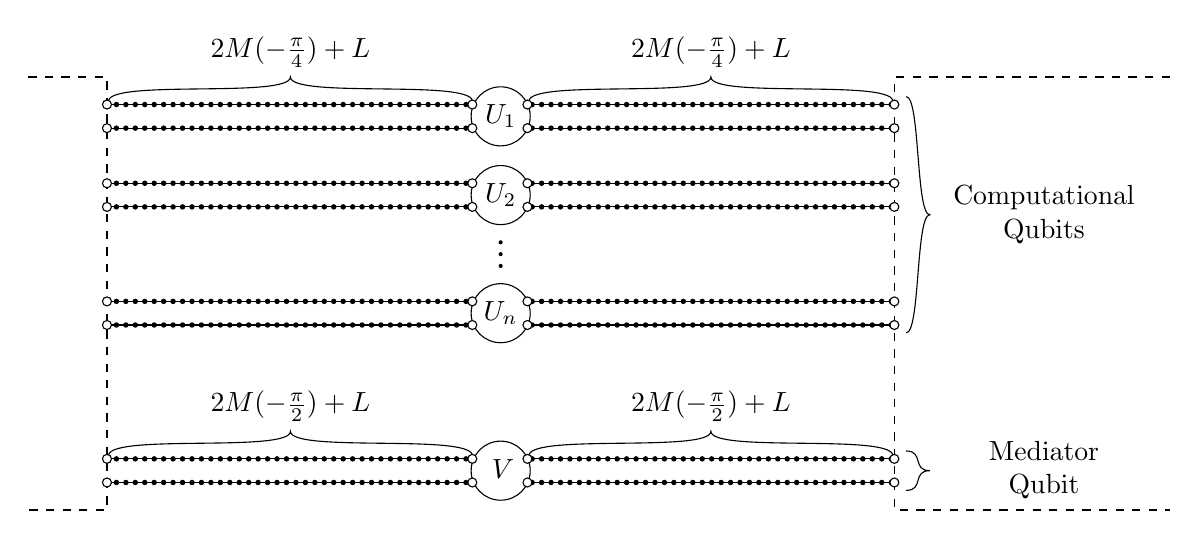
\begin{tikzpicture}[
  unitary/.style={circle,draw=black,fill=white,
    inner sep=0pt,minimum size=7.5mm},
  dots/.style={circle,fill=black,
    inner sep=0pt,minimum size=1.5pt},
  vert/.style={circle,fill=black,
    inner sep=.7pt,minimum size=0pt},
  attach/.style={circle,draw=black,fill=white,inner sep=1.15pt,minimum size=0}]

  \foreach \n /\y in {U_1/2.5,U_2/1.5,U_n/0,{V_{\med}}/-2}{
    \begin{scope}[yshift = \y cm]
      \foreach \x in {0,.12,...,10} {
        \node at (\x, -.15) [vert] {};
        \node at (\x, .15) [vert] {};
      }
      \draw (0, -.15) to (10, -.15);
      \draw (0,  .15) to (10,  .15);
      \node at (5,0) [unitary]{$ \n $};


    \end{scope}
  }
  
  \foreach \x in {0,5.34}{
  \foreach \y /\p in {2.5/4,-2/2}{
  \begin{scope}[xshift=\x cm,yshift=\y cm]
    \node (\x\p) at (2.33,.5)[above] {$2M(-\frac{\pi}{\p}) + L$};
  
    \draw (0.02,0.2) to[out=80,in=-90,looseness=0.3] (2.33,.5)
                     to[out=-90,in=100,looseness=0.3] (4.64,.2);
  \end{scope}}} 
                  
  \draw (10.15,2.75) to[out=0,in=-180,looseness=0.3] (10.45,1.25)
                    to[out=-180,in=0,looseness=0.3] (10.15,-.25);
  \node at (11.9,1.25)
      {\begin{tabular}{c}
          Computational\\ 
          Qubits\end{tabular}};


  \draw (-1,3) to (0, 3) to (0,-2.5) to (-1,-2.5) [dashed];
  \draw (13.5,3) to (10,3) to (10,-2.5) to (13.5,-2.5) [dashed];

  \node at (5,.9) [dots] {};
  \node at (5,.75)    [dots] {};
  \node at (5,.6) [dots] {};

  \draw (10.15,-1.75) to[out=0,in=-180,looseness=1.5] (10.45,-2)
                    to[out=-180,in=0,looseness=1.5] (10.15,-2.25);
  \node at (11.9,-2) 
      {\begin{tabular}{c}
          Mediator\\ 
          Qubit\end{tabular}};
          
   \foreach \x in {0, 10, 4.64, 5.34}{
   \foreach \y in {2.35,2.65,1.65,1.35,.15,-.15,-1.85,-2.15}{
     \node at (\x, \y) [attach] {};
   }}
\end{tikzpicture}
  \caption{The intuitive idea for a single-particle block.}
  \label{fig:SP_block}
\end{figure}
  
With this construction, we have exactly the same idea as in the \sec{single_qubit_multi_gate_computation} to analyze the time-evolution of a particular initial logial state, and the analysis proceeds accordingly.  If we use \lem{truncation} to only use the vertices close to a the wavepacket (and in particular the nearest copy of $G_{V_j}^{U_j}(K)$) we can use \cor{multi_qubit_single_gate_encoded_computation} to approximate the evolution.
  
  
Concretely, let us choose some cutoff length $L$, set $\sigma = \frac{L}{2\sqrt{\log L}}$, chose $\mu = 2L$ and $K = 2\mu$ and $T = \frac{\mu}{\sin |k|}$.  With these choices, our initial logical state will be nearly identical to \eq{single_qubit_input_encoding}, but where the basis states also have a label corresponding to fact that there are multiple long paths:
\begin{align}
  \ket{z}_{\text{log},\text{in}} = \gamma \sum_{x = \mu - L}^{\mu + L} e^{ i k x} e^{ - \frac{(x-\mu)^2}{2\sigma^2}} \ket{x,z+1,1}.
\end{align}
In a similar manner, the final state of the qubit will be defined as
 \begin{align}
  \ket{z}_{\text{log},\text{out}} = \gamma e^{- 2 i Tg \cos k} \sum_{x = \mu - L}^{\mu + L} e^{ -i k x} e^{ - \frac{(x-\mu)^2}{2\sigma^2}} \ket{x,z+2^{n}+1,g},
\end{align}
Additionally, we will need to define logical states at several times throughout the computation, corresponding to the states after each applied unitary.  As such, we will define the logical state after the $j$th scattering event (and before the $(j+1)$th scattering event) as
\begin{align}
  \ket{z}_{\text{log},j} &= \gamma e^{-2i Tj \cos k}\sum_{x = \mu - L}^{\mu + L} e^{ i k x} e^{ - \frac{(x-\mu)^2}{2\sigma^2}} \ket{x,z+1,j+1} \\
  &= \gamma e^{- 2 i Tj \cos k} \sum_{x = \mu - L}^{\mu + L} e^{ -i k x} e^{ - \frac{(x-\mu)^2}{2\sigma^2}} \ket{x,z+2^n+1,j}.
\end{align}

\todo{make the words work}
\begin{align}
  &\Big \Vert e^{ i A(G_{\mathcal{C}} )g T} \ket{\psi}_{\text{log},\text{in}} - \ket{U_{\mathcal{C}} \psi}_{\text{log},\text{out}}\Big \Vert\nonumber\\
  & \qquad \leq \sum_{j = 0}^{g-1} \Big \Vert e^{ i A(G_{\mathcal{C}})T} \ket{U_{j} U_{j-1}\cdots U_1 \psi}_{\text{log},j} - \ket{U_{j+1}U_{j} \cdots U_1 \psi}_{\text{log},j+1}\Big \Vert
\end{align}
Note that each individual term is close to that in \lem{single_qubit_encoded_computation}, but where the Hamiltonian is given by $A(G_{\mathcal{C}})$ as opposed to $A(G(K))$.  However, we can use \lem{truncation}, with $H = A(G_{\mathcal{C}})$, $\tilde{H} = G(K-1)$,  $N_0 = \frac{\mu}{4}$, and the error $\delta$ from \lem{single_qubit_encoded_computation}, we have that for all logical states $\ket{\phi}$,
\begin{align}
   &\Big \Vert e^{ i A(G_{\mathcal{C}})T} \ket{\phi}_{\text{log},j} - \ket{U_{j+1}\phi}_{\text{log},j+1}\Big \Vert\nonumber\\
   &\leq \Big(\frac{ 16 e \norm{A(G_{\mathcal{C}})} T}{\mu} + 2\Big)\bigg[ \xi \sqrt{\frac{\log L}{L}} + 2^{- \mu + L +2} \bigg(1 -   \chi \sqrt{\frac{\log L}{L}} \bigg)\bigg]\\
   & \leq \kappa_j \sqrt{\frac{\log L}{L}},
\end{align}
where $\kappa$ is depends on $k$ and the maximum degree of $G_{\mathcal{C}}$ (which we assume to be constant).  We can then see that
\begin{align}
  &\Big \Vert e^{ i A(G_{\mathcal{C}} )g T} \ket{\psi}_{\text{log},\text{in}} - \ket{U_{\mathcal{C}} \psi}_{\text{log},\text{out}}\Big \Vert\nonumber\\
  & \qquad \leq \sum_{j = 0}^{g-1} \Big \Vert e^{ i A(G_{\mathcal{C}})T} \ket{U_{j} U_{j-1}\cdots U_1 \psi}_{\text{log},j} - \ket{U_{j+1}U_{j} \cdots U_1 \psi}_{\text{log},j+1}\Big \Vert\\
  &\qquad \leq g\kappa \sqrt{\frac{\log L}{L}}.
\end{align}
As such, if we take $L$ larger than $g^2\kappa^2$ we find that the error can be made arbitrarily small.

\todo{figure out product log stuff}


%%%%%%%%%%%%%%%%%%%%%%%%%%%%%%%%%%%%%%%%%%%%%%%%%%%%%%%%%%%%%%%%%


\section{Universality via single-particle scattering}

With our results so far, we technically haven't yet shown that our results are 

Now that we know that the time-evolution of a particular state on a sparse (and efficiently computable) graph can be used to simulate an arbitrary quantum circuit, to show that such computation is universal for quantum computation we need to show the simulation in the other direction.  This is not particularly difficult, but is a necessary step.

In particular, let us discuss the problem of
\begin{problem}[\QWE] Given a $d$-sparse, row-computable simple graph $G$ on $\Theta(2^n)$ vertices, an efficiently preparable initial state $\ket{\phi_{\text{init}}^G}$, a subset of the vertices $\mathcal{V}_{\text{accept}}$ (for which membership is easily verified), and a time $T \in \poly(n)$, determine whether
\begin{itemize}
   \item $\bra{\phi_{\text{init}}^G} e^{i A(G) T} \Pi_{\mathcal{V}} e^{-i A(G)T} \ket{\phi_{\text{init}}^G} \geq \frac{2}{3}$, or
   \item $\bra{\phi_{\text{init}}^G} e^{i A(G) T} \Pi_{\mathcal{V}} e^{-i A(G)T} \ket{\phi_{\text{init}}^G} \leq \frac{1}{3}$,
\end{itemize}
where we are guaranteed that one case holds.
\end{problem}

Note that the efficient preparation of $\ket{\phi_{\text{init}}^G}$, and the fact that membership $\mathcal{V}$ is easily verified, are used to insure that the bulk of the computational power arises from the time evolution on $G$, and that we are not hiding the computation in the preparation of the initial state or in our measurements.

\subsection{Simulation of a quantum circuit}

Let us first show that an arbitrary quantum circuit can be simulated by the time evolution of an efficiently specifiable state on a succinctly represented graph.  This is the point at which we will use our graph scattering techniques.  

In particular, choose some $k\in (-\pi,0)$ for which we have a universal set of quantum scattering gates are known (such as those in \sec{explicit_encodings}, and let $\mathcal{C}_x$ be a circuit corresponding to the circuit verification problem instance $x$, such that $\mathcal{C}_x$ can be decomposed into a sequence of one- and two-qubit gates from the universal gate set $\mathcal{S}_{k}$ and controlled-not gates (as defined in \sec{explicit_encodings}).  We assume that the circuit $\mathcal{C}_x$ acts on $m$ qubits (where $m\in \poly(n)$), and that the circuit satisfies:
\begin{itemize}
  \item if $x\in$ \QCircVer, then $\pr(\mathcal{C}_x,0^m) > 1-2^{-|x|}$,
  \item if $x\notin$ \QCircVer, then $\pr(\mathcal{C}_x,0^m) < 2^{-|x|}$.
\end{itemize}
In other words, with high probability the circuit $\mathcal{C}_x$ computes whether the instance $x$ is in \QCircVer.

Note that we almost have from \sec{multi_qubit_computations} that such a simulation is possible, we just need to ensure that the unitary $\mathcal{C}_x$ has the decomposition required, that the associated graph is $d$-sparse and row-computable, that the initial state is efficiently preparable, and that the subset of vertices corresponding to an accepting computation is easily verifiable.

For the first problem, note that we can easily change the circuit $\mathcal{C}_x$ into a circuit of the form described in \sec{multi_qubit_computations} by doubling the number of unitaries in the circuit.  In particular, if $\mathcal{C}_x = U_g U_{g-1} \cdots U_{1}$, the quantum walk will simulate the circuit $\mathcal{D}_x = V_g V_{g-1} \cdots V_1$, where 
\begin{align}
  V_j = \begin{cases}
    U_j \II^{(1)}_{2} & U_j \text{ is a 2-qubit gate}\\
    \II_{4}^{(1,2)} U_j & U_j \text{ is a 1-qubit gate}.
  \end{cases}
\end{align}
In this manner, $\mathcal{D}_x$ is an alternating sequence of $1$- and $2$-qubit gates.  For a given $L$, we can thus use the construction of \sec{multi_qubit_computations} for the graph $\mathcal{D}_x$.

To see that the Hamiltonian corresponding to $G_{\mathcal{D}_x}(K)$ is $d$-sparse and row-computable, note that the Hamiltonian simply corresponds to the adjacency matrix of the graph.  As such, the sparsity is exactly equal to the maximum degree of the graph, which is bounded by some constant $\dmax$, which depends on the scattering gadgets for the momentum $k$. 

To see that the graph is row-computable, note that our construction already gives us the ability to efficiently determine the neighbors of a vertex. In the labeling scheme given, vertices along each path are labeled according to the basis state it corresponds to, the number of scattering gadgets to it's left, and the position along the gadget, and are only connected to vertices the two vertices with positions that differ by 1.  The vertices contained in a copy of $\widehat{G}_j$ for some graph scattering gadget $j$ are labeled by the computational state of the qubits not affected by the corresponding unitary, along with the labeling of the graph $\widehat{G}_j$, and are only connected to those vertices with the same labeling of gadget and are connected in $\widehat{G}_j$.  The only difficulties are the terminal gadgets, but these are easily determined since we only ever apply either the identity gate or a controlled not to the logical state of the corresponding input/output terminals.  Hence, the Hamiltonian for the graph is $\dmax$-sparse and row-computable.

For the initial state, note that the construction of \sec{multi_qubit_computations} only has non-zero amplitude on $2L + 1$ vertices, which only depends on $\mathcal{C}$ in terms of the length.  This is both efficiently specifiable and easily constructed.

Finally, we have that the states corresponding to an accepting computation are easy to check; they are simply those vertices on the final ($g+1$) long paths with the first qubit in logical state 1. 

Putting this together, we can then use the results of \sec{multi_qubit_computations} to show that any \QCircVer instance can be reduced to an instance of \QWE.  Hence, \QWE  is \BQP-hard.



\subsection{Simulation of a quantum walk}

Let us now show that \QWE is in \BQP.  It relatively easily follows from \thm{Hamiltonian_simulation}, since we simply need to evolve a given Hamiltonian for the time $T$, and then measure in the computational basis.

In particular, the fact that the initial state is efficiently preparable means that there exists a quantum circuit $\mathcal{C}_{\text{prep}}$ that prepares the given initial state from the state $\ket{0^n}$, possibly including some ancilla states.  Moreover, the quantum circuit only consists of $\poly(|x|)$ one- and two-qubit gates, since the state is efficiently preparable.  (Note that this bound depends on the efficiency of the given instance.)

From the initial state, we can then use \thm{Hamiltonian_simulation} to evaluate the quantum walk Hamiltonian for the time $T$.  Since the Hamiltonian is $d$-sparse, and since the Hamiltonian is an adjacency matrix, we have that its maximal eigenvalue is at most $d$.  Assuming that we want to perform the simulation with error $1/10$, we can then simulate the evolution of the quantum walk in an efficient manner.  (Again, the efficiency depends on the given instance.)

Finally, the quantum circuit can measure the state of the system in the vertex basis.  If the measured vertex belongs to $\mathcal{K}$ (a post-processing procedure that can be done efficiently), then the circuit accepts.  Otherwise, the circuit rejects.

As the quantum walker fails with probability at most $\frac{1}{3}$ (i.e., accepts the state for a yes instance with probability at least $\frac{2}{3}$, and accepts a no-instance with probability at most $\frac{1}{3}$), with the error arising from the simulation we still have that the yes and no instances of our simulations have a constant acceptance gap.  Hence, we have that \QWE is in \BQP.

Put together with our results using scattering, we then have that \QWE is \BQP-complete, or that quantum walks are universal for quantum computation.

%%%%%%%%%%%%%%%%%%%%%%%%%%%%%%%%%%%%%%%%%%%%%%%%%%%%%%%%%%%%%%%%%

\section{Discussion and extensions}

Note that these results are essentially already known.  In particular, Childs gave a similar result using scattering theory, but where his time evolution arose from the theory of stationary phases. 

One key point in this analysis is that, while we can reduce the graph to be degree-3, without changing much except the individual gadgets, the permutation of the underlying paths plays a key part in our encoded gates.  However, these permutations are intrinsically non-planar (assuming that there are more than three non-identity 2-qubit gates).  One might ask whether \text{any} planar graph could be used to encode a computation, or whether non-planarity is required for the computations.

Additionally, our current construction assumes no errors, and has no error-correction easily built in.  We are unsure how error correction could be implemented in this scheme, since both non-local measurements and measurements in the middle of the computation seem rather difficult.  This might also help us in the next chapter, where we use similar methods to show the universality of multi-qubit quantum walks.

%%%%%%%%%%%%%%%%%%%%%%%%%%%%%%%%%%%%%%%%%%%%%%%%%%%%%%%%%%%%%%%%%

\biblio

\end{document}